\documentclass[12pt]{article}
%\documentclass{article}

\usepackage{times}
\usepackage[final]{graphicx}
\usepackage{hyperref}

\setlength{\topmargin}{-0.5in}
\setlength{\oddsidemargin}{0in}
\setlength{\evensidemargin}{0in}
\setlength{\textwidth}{6.5in}
\setlength{\textheight}{9.0in}

\begin{document}

\centerline{\bf \Large CS295/CS395/CSYS395: \href{CS295_395_Syllabus.pdf}{\underline{Evolutionary Robotics}}}

\vspace{0.5cm}

\centerline{\bf \large Programming Assignment 3 of 10}

\vspace{0.5cm}

\centerline{\large Assigned: Friday, September 16, 2011}

\vspace{0.5cm}

\centerline{\large Due: Friday, September 23, 2011 by midnight}

\vspace{0.5cm}

\noindent \textbf{Description:} In this assignment you will apply the hillclimber you developed in assignment 1 to the artificial neural networks (ANNs) you developed in assignment 2. The program you develop in this assignment works as follows:

\begin{enumerate}

\item Create a (numNeurons=)$10$ $\times$ $10$ (numNeurons=)matrix, parent, to hold the synapse values for an ANN with numNeurons=10 neurons.

\item Randomize the parent synapse matrix.

\item Create a (numUpdates=)$10$ $\times$ (numNeurons=)$10$ matrix neuronValues to hold the values of the neurons as the network is updated. The first row stores the initial values of the neurons, which for this assignment will all initially be set to 0.5. The second row will store the new values of each neuron, and so on.

\item Create a vector of length 10, desiredNeuronValues, that holds the output that we want the ANN to create. We'll compare the final values of the neurons---the last row of neuronValues---to this vector. The closer the match, the higher the fitness of parent synapse matrix.

\item Update neuronValues nine times (thus filling in rows two through 10) using the parent synapse values.

\item The program will then loop through 1000 generations. For each loop: \\
.\hspace{1cm}Create the child synapse matrix by copying and perturbing the parent synapse matrix.\\
.\hspace{1cm}Set each element in the first row of neuronValues to 0.5.\\
.\hspace{1cm}Update the neuronValues of the ANN nine times using the child synapse values.\\
.\hspace{1cm}Calculate and save the fitness of the child synapses as childFitness.\\
.\hspace{1cm}If the childFitness is better than parentFitness, replace the parent synapse matrix with the child synapse matrix and set parentFitness to the childFitness value.

\end{enumerate}

Here are the steps to implement the program.

\begin{enumerate}

\item \textbf{Back up your Python code from assignment 2.} Encapsulate your code from assignment 2 in a single file, Assignment\_2.py, such that when you run it you can reproduce all of the visualizations from that assignment. This will prove to you that that code is working fine, as you will use it in this and subsequent assignments.

\item Create a blank Python file called Assignment\_3.py. As you implement this assignment, copy and paste functions from assignments 1 and 2 as they are needed.

\item Copy and paste the main function that you created in assignment 1 at step 8, comment out all but the first two lines and change it so that instead of creating a vector of random numbers, you create a matrix of random numbers. This matrix contains the synaptic weights of the parent neural network. (You'll have to copy across the \textbf{\texttt{MatrixCreate}} and \textbf{\texttt{MatrixRandomize}} functions from that assignment as well.) Note that in Python, putting a hash symbol (\#) at the front of the line comments it out:

\textbf{\texttt{parent = MatrixCreate(10,10)}}\\
\textbf{\texttt{parent = MatrixRandomize(parent)}}\\
\# \textbf{\texttt{parentFitness = Fitness(parent)}}\\
\# \textbf{\texttt{for currentGeneration in range(0,1000):}}\\
\# \indent \textbf{\texttt{\hspace{1cm}print currentGeneration, parentFitness}}\\
\# \indent \textbf{\texttt{\hspace{1cm}child = MatrixPerturb(parent,0.05)}}\\
\# \indent \textbf{\texttt{\hspace{1cm}childFitness = Fitness(child)}}\\
\# \indent \textbf{\texttt{\hspace{1cm}if ( childFitness > parentFitness ):}}\\
\# \indent \textbf{\texttt{\hspace{2cm}parent = child}}\\
\# \indent \textbf{\texttt{\hspace{2cm}parentFitness = childFitness}}\\

\item Insert a \textbf{\texttt{print parent}} statement after the two lines to make sure the matrix was randomized correctly.

\item Modify the MatrixRandomize function so that it returns values in [-1,1] rather than [0,1]. \textbf{\texttt{parent}} now encodes synaptic weights for a neural network with 10 neurons. \textbf{\texttt{print parent}} to make sure this was done correctly.

\item Uncomment the third line, and copy across the \textbf{\texttt{Fitness}} function you created in assignment 1.

\item You must now modify the \textbf{\texttt{Fitness}} function so that it returns a single value that indicates the fitness, or quality of the neural network specified by the synaptic weights stored in \textbf{\texttt{parent}}. Steps 7 through 14 will help you to do this. First, delete all the code currently within the \textbf{\texttt{Fitness}} function, and add code into the now-empty function that creates an all-zero (numUpdates=)$10$ $\times$ (numNeurons=)$10$ matrix \textbf{\texttt{neuronValues}} like you did in assignment 2. Print the matrix to make sure it is correct.

\item Fill each element in the first row of \textbf{\texttt{neuronValues}} with $0.5$: each of the 10 neurons will start with this value. \textbf{\texttt{print neuronValues}} to make sure this was done correctly.

\item Copy across the \textbf{\texttt{Update}} function you developed in assignment 2, step 12. Use it to fill in the second row of \textbf{\texttt{neuronValues}} using the synaptic weights stored in parent. Apply it again to fill in the third row. Apply it nine times in total so that \textbf{\texttt{neuronValues}} is completely filled (\textbf{\texttt{numUpdates=10}} in this assignment). Print \textbf{\texttt{neuronValues}} periodically to make sure it is being updated correctly (i.e. each row of zeros are replaced by non-zero values).

\item After the nine calls to \textbf{\texttt{Update}}, use the plotting function you developed in assignment 2, step 13 to print out how the neuron values change over time. You should get a picture like Fig. \ref{Fig}a or d.

\item Now we are going to calculate how close the final set of neuron values is to some desired set of neuron values. After \textbf{\texttt{neuronValues}} has been filled, extract the last row as follows: \textbf{\texttt{actualNeuronValues = neuronValues[9,:]}}. This copies the last row of \textbf{\texttt{neuronValues}}.

\item Create a vector that stores the desired values for the neurons. Let's select for odd-numbered neurons that are on, and even-numbered neurons that are off:

\textbf{\texttt{desiredNeuronValues = VectorCreate(10)}}\\
\textbf{\texttt{for j in range(0,10,2):}}\\
\indent \textbf{\texttt{\hspace{1cm}desiredNeuronValues[j]=1}}\\

\item \textbf{\texttt{VectorCreate}} returns a row vector of length 10. To create this function, copy, rename and modify \textbf{\texttt{MatrixCreate}}. To create a vector using NumPy: \textbf{\texttt{v = zeros((width),}} \textbf{\texttt{dtype='f')}}. The for loop counts from 0 to 9 in steps of 2: 0,2,4,... This code should produce a vector of the form [1,0,1,0,1,0,1,0,1,0].

\item Now, create a function \textbf{\texttt{MeanDistance(v1,v2)}} that returns the normalized distance between two vectors with elements between 0 and 1: The function should return 0 if the vectors are the same, and 1 if they are maximally different. This function should be used to compute the distance $d$ between \textbf{\texttt{actualNeuronValues}} and \textbf{\texttt{desiredNeuronValues}}. \textbf{\texttt{Fitness}} should then return $f=1-d$: the lower the distance between the vectors, the closer the fitness approaches 1.

\item Now, uncomment the remaining lines of the main function, and ensure that your hillclimber is working correctly: \textbf{\texttt{child}} should be a slightly different matrix compared to \textbf{\texttt{parent}}, and \textbf{\texttt{parentFitness}} should increase toward 1 as the loop runs.

\item Add a fitness vector to the main function, and record \textbf{\texttt{parentFitness}} into this vector after each pass through the loop.

\item Add in a call to your neural network plotting function just before the main loop begins, to show the behavior of the initial random network. Copy and paste the resulting image into your document, which should look like Fig. \ref{Fig}a or d. Note that the image should show a band of gray at the top, which correspond to the initial 0.5 settings of all the neurons.

\item Add another call to the plotting function after the main loop has finished, to show the behavior of the final, evolved neural network. Copy and paste this figure into your document. It should show an alternating pattern of black and white pixels in the bottom row, like Fig. \ref{Fig}b. It may not be perfectly alternating if the fitness of that run did not get to a fitness of 1; this is fine if this is the case.

\item Store the fitness of the parents as the main loop iterates in a vector, and plot that vector. It should look like Fig. \ref{Fig}c. Copy it into your document. Run the program a few times to see what kinds of patterns you get.

\item Now copy the \textbf{\texttt{Fitness}} function, rename it \textbf{\texttt{Fitness2}}, and change the two calls to \textbf{\texttt{Fitness}} in your main function to calls to \textbf{\texttt{Fitness2}}.

\item Leave the internals of \textbf{\texttt{Fitness2}} as they are, but change how the fitness of the neural network's behavior is calculated. Remove the mean squared error calculation, and instead compute the average difference between neighboring elements in the matrix: \\
\textbf{\texttt{diff=0.0}}\\
\textbf{\texttt{for i in range(0,9):}}\\
\indent \textbf{\texttt{\hspace{1cm}for j in range(0,9):}}\\
\indent \textbf{\texttt{\hspace{2cm}diff=diff + abs(neuronValues[i,j]-neuronValues[i,j+1])}}\\
\indent \textbf{\texttt{\hspace{2cm}diff=diff + abs(neuronValues[i+1,j]-neuronValues[i,j])}}\\
\textbf{\texttt{diff=diff/(2*9*9)}}

\item Re-run the hillclimber, and save out the initial random neural network's behavior (as in Fig. \ref{Fig}d), the behavior of the final, evolved neural network (as in Fig. \ref{Fig}e), and the fitness increase during the hillclimber (as in Fig. \ref{Fig}f). Note that the evolved neural network may not reach a perfect checkerboard configuration; that is fine if this is the case. Run the program a few times to see what kinds of patterns you get.

\item \textbf{Things to think about:} What other kinds of neural behavior could you select for? What visual pattern would it produce when plotted? If you like, try implementing these new fitness functions and see whether you get the pattern you were expecting. Answers to these questions need not be included in the document you hand in.

\end{enumerate}

\begin{figure}[!t]
\centerline{
a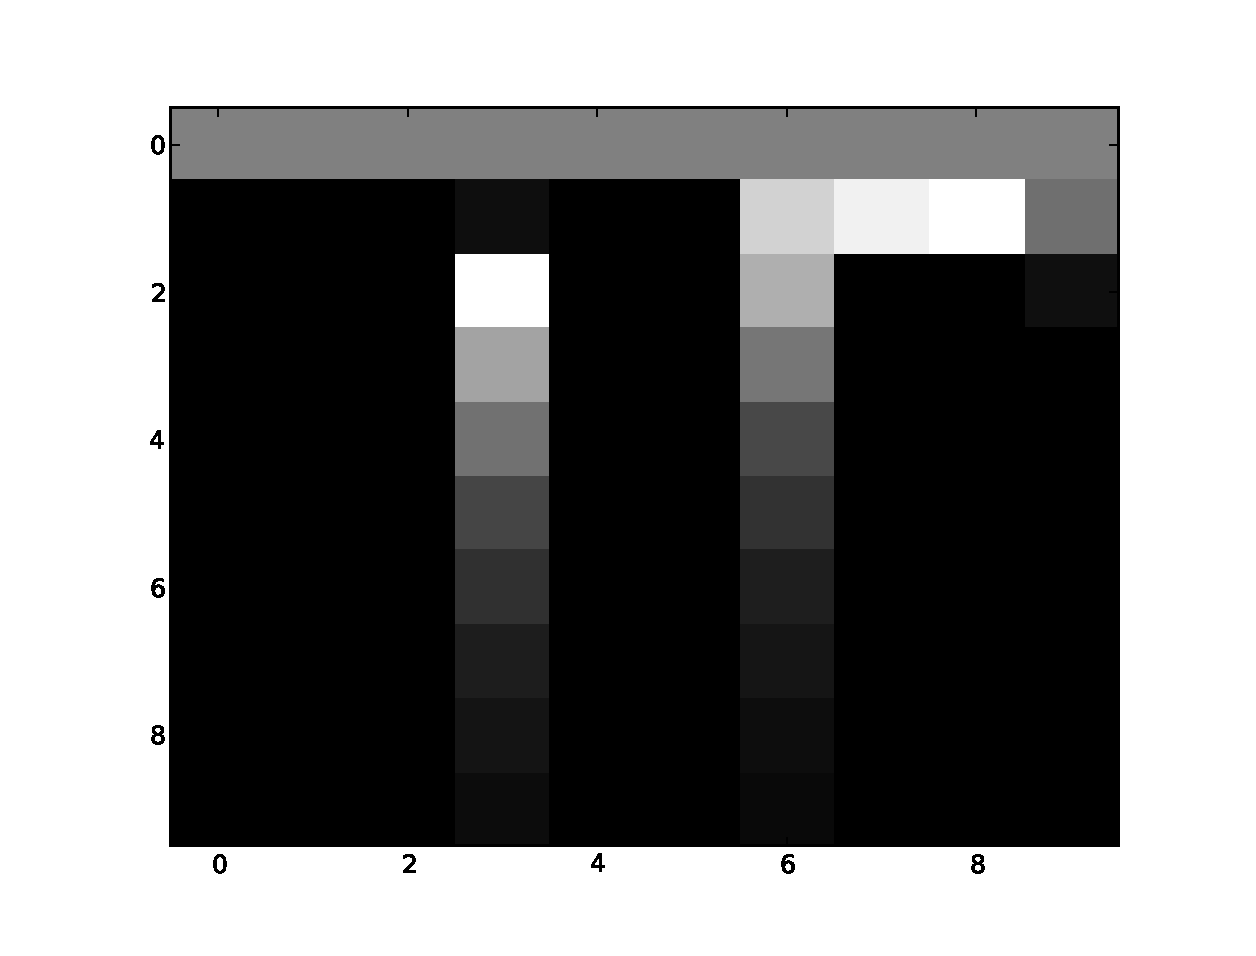
\includegraphics[width=0.32\textwidth]{Fig1a.eps}
b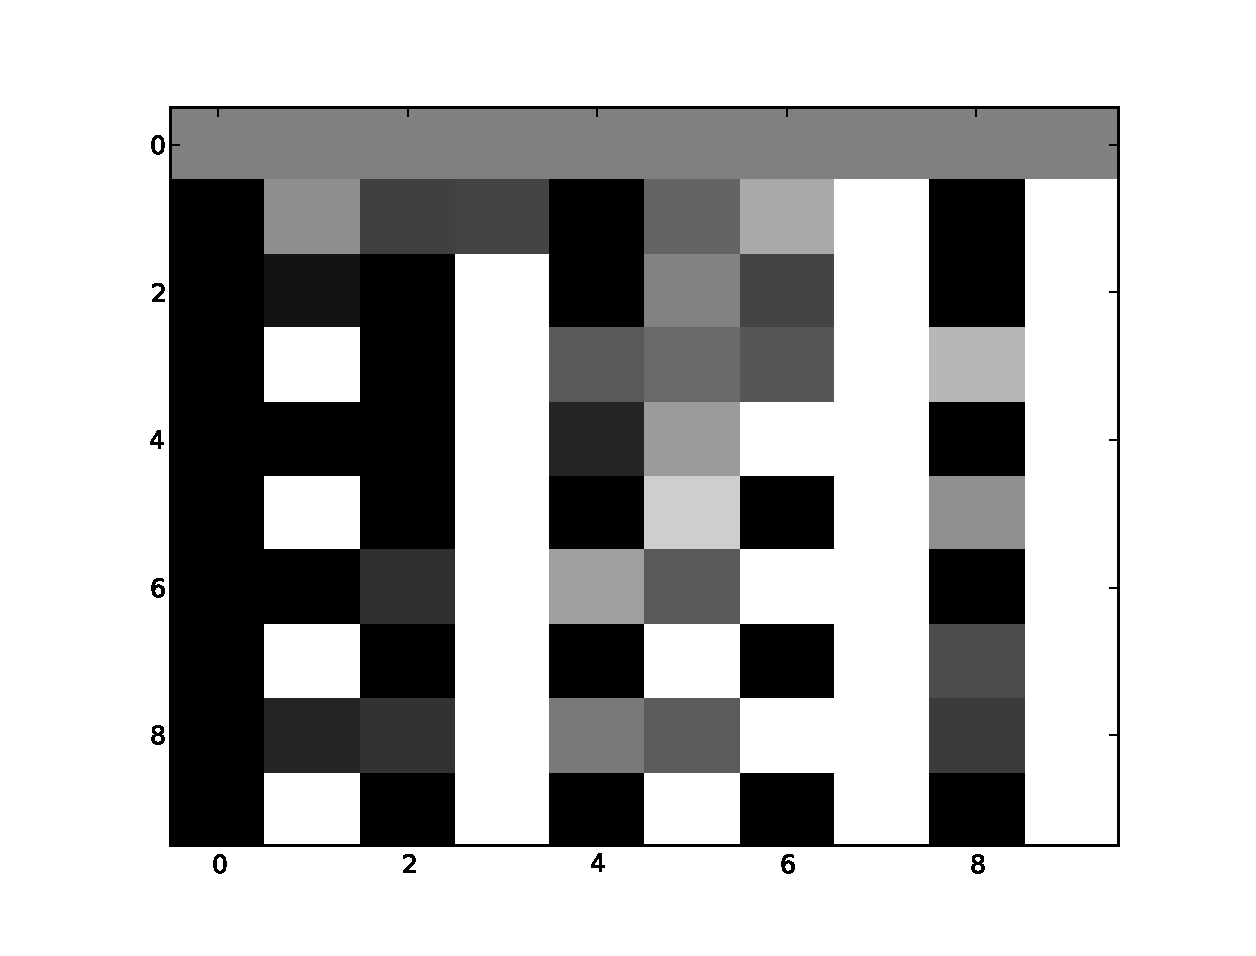
\includegraphics[width=0.32\textwidth]{Fig1b.eps}
c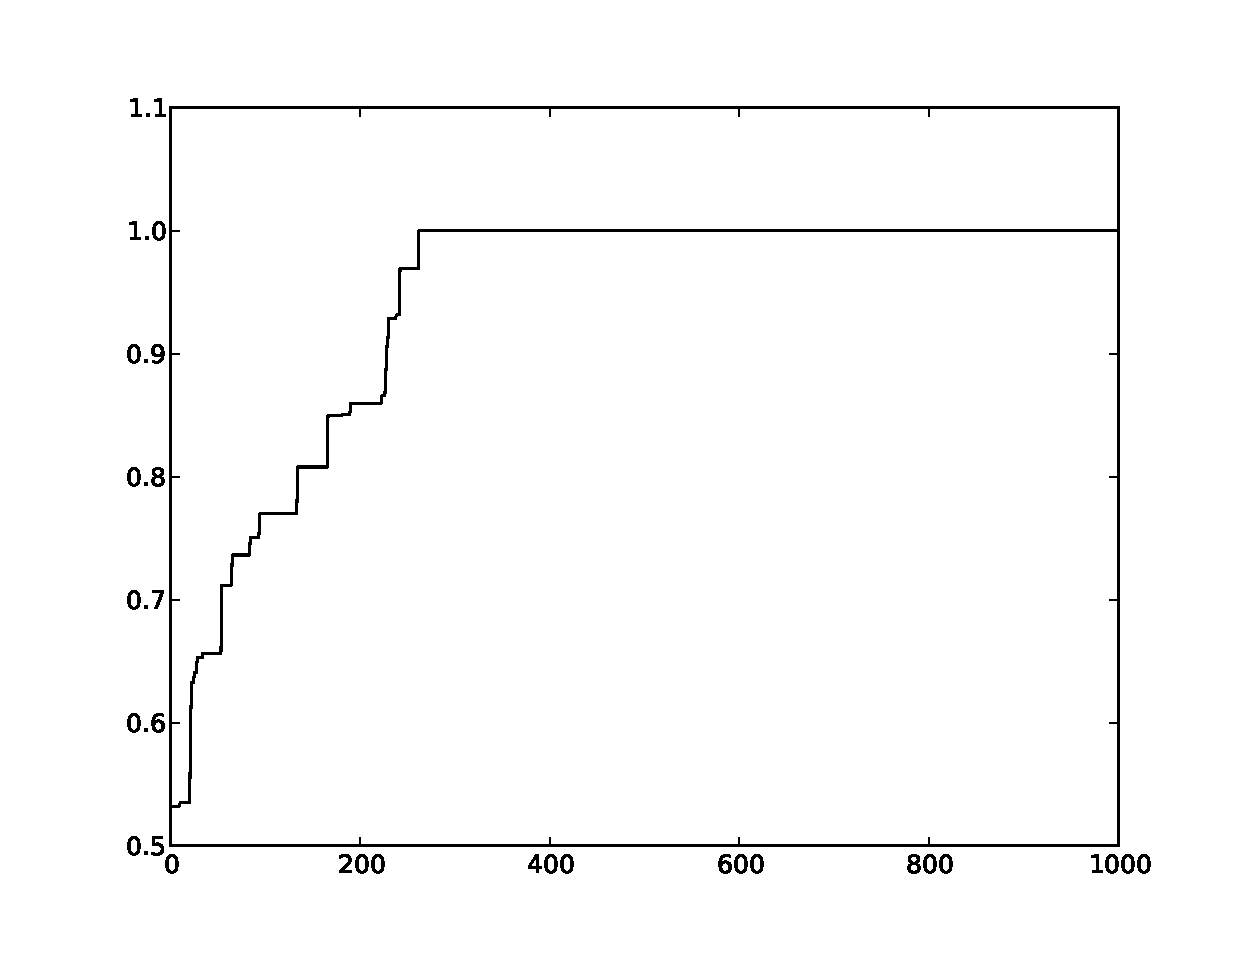
\includegraphics[width=0.32\textwidth]{Fig1c.eps}
}
\centerline{
d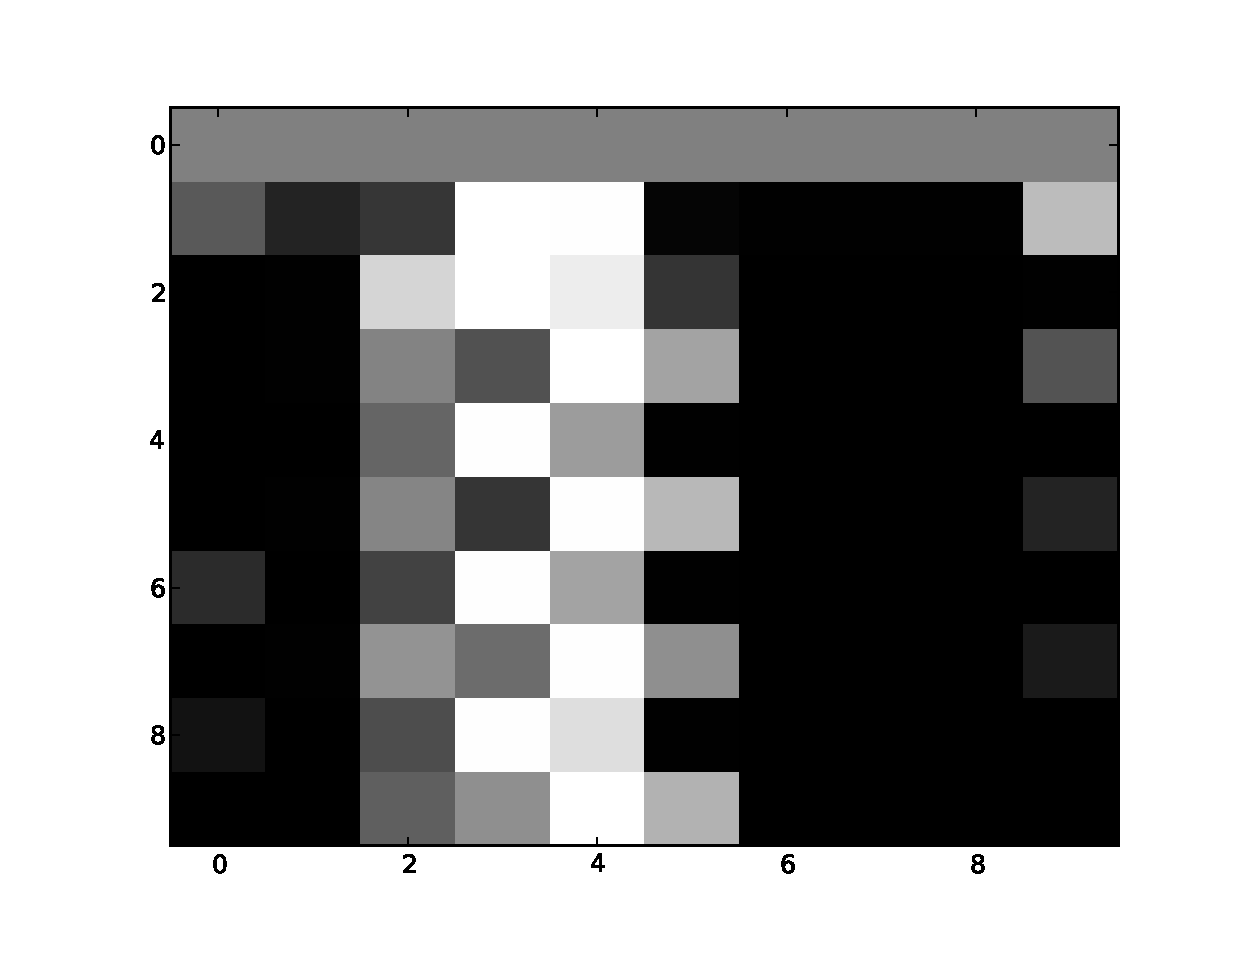
\includegraphics[width=0.32\textwidth]{Fig1d.eps}
e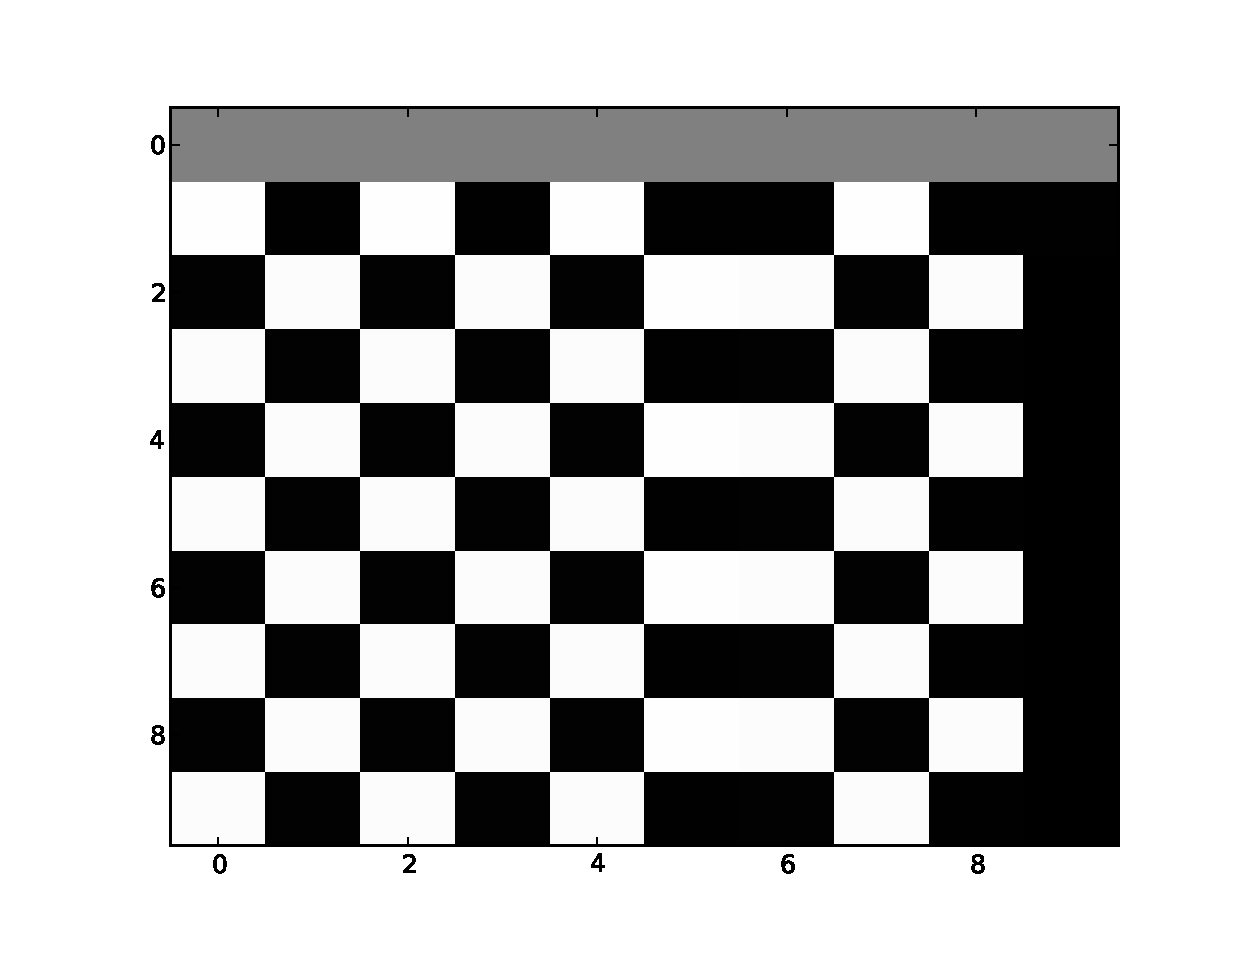
\includegraphics[width=0.32\textwidth]{Fig1e.eps}
f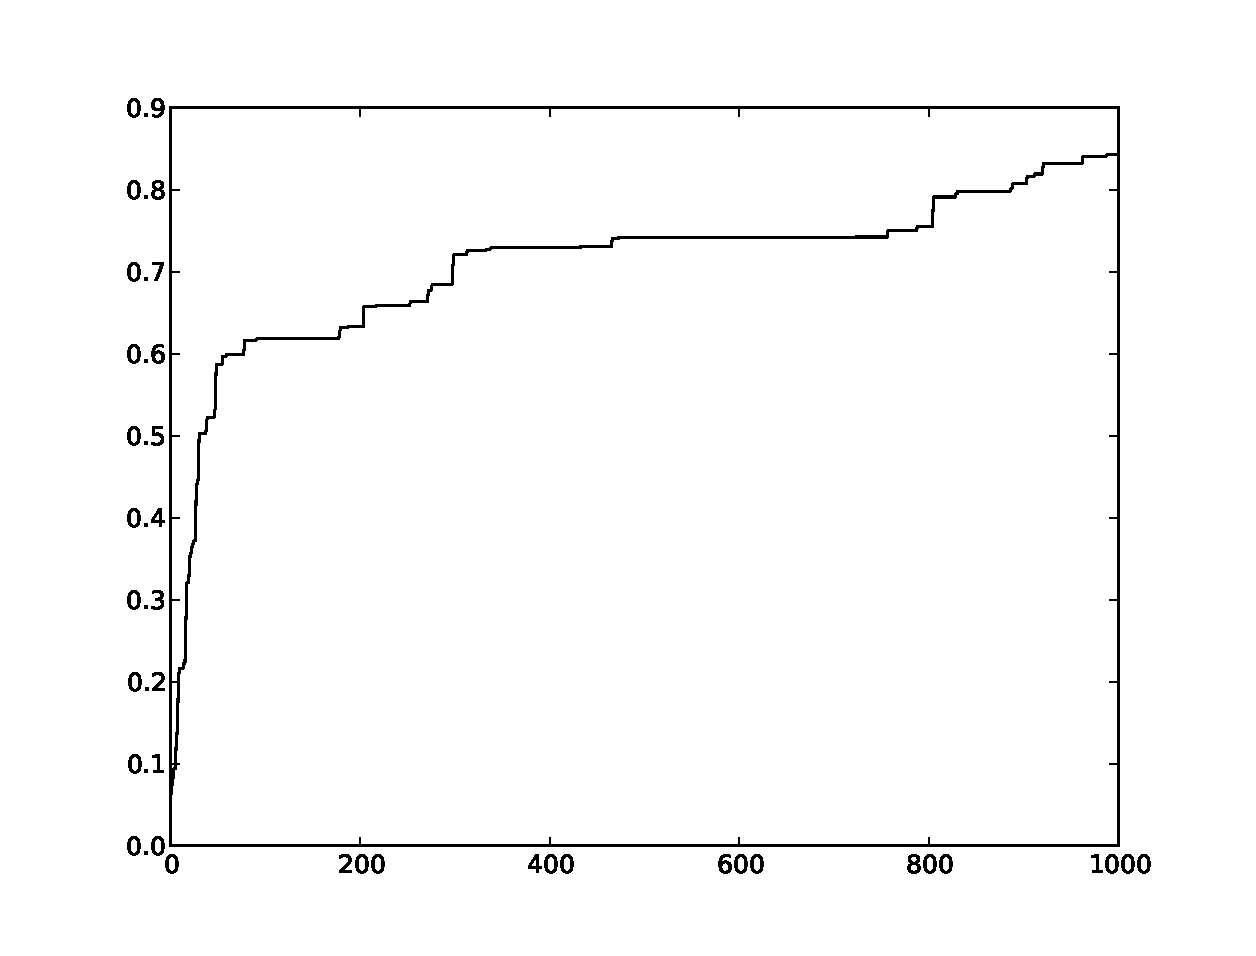
\includegraphics[width=0.32\textwidth]{Fig1f.eps}
}
\caption{Visualizations demonstrating the successful evolution of artificial neural networks.
a: Behavior of an initial, random ANN.
b: Behavior of an ANN evolved such that the neuron values, on the last update (bottom row), show alternating patterns ($n_1$=0,$n_2$=1,$n_3$=0,...).
c: The fitness change of the best ANN over evolutionary time.
d: Behavior of an initial, random ANN from another evolutionary run.
e: Behavior of an ANN evolved such that neighboring neurons exhibit different values, and those values change from one time step to the next.
f: The fitness change of the best ANN over evolutionary time using this second fitness function.
}
\label{Fig}
\end{figure}

\end{document} 